% Copyright 2021 Thomas Ascher
% SPDX-License-Identifier: CC-BY-SA-4.0

\documentclass[a4paper,parskip=half]{scrartcl}

\usepackage[T1]{fontenc}
\usepackage[ngerman]{babel}
\usepackage{csquotes}
\usepackage[regular,condensed,sfdefault]{roboto}
\usepackage{booktabs}
\usepackage{graphicx}
\usepackage{float}
\usepackage[hidelinks,pdfencoding=auto,
  pdfauthor={Thomas Ascher},
  pdfusetitle,
  pdfkeywords={Grainfather,Conical Fermenter,Pro Controller}]{hyperref}
\usepackage{microtype}

\addto\extrasngerman{
\def\figureautorefname{Abb.}
\def\tableautorefname{Tab.}
\def\equationautorefname{Gl.}
}

\addto\captionsngerman{
\renewcommand{\figurename}{Abb.}
\renewcommand{\tablename}{Tab.}
}

\title{Grainfather Conical Fermenter Pro Controller}
\author{Thomas Ascher <thomas.ascher@gmx.at>}
\date{09. Oktober 2021, \href{http://creativecommons.org/licenses/by-sa/4.0/}{CC BY-SA 4.0}}

\begin{document}
\maketitle

\section*{Einleitung}

Mittlerweile stehen dem Heimbrauumfeld eine breite Auswahl von Instrumenten
mit verschiedenen Messprinzipien zur Verfügung, die es ermöglichen, den
Alkoholgehalt eines selbst gebrauten Biers abzuschätzen oder den
Gärverlauf zu beobachten. Das ist neben der klassischen Bierspindel
unter anderem das Handrefraktometer. Die Refraktometrie ist
kein Neuling im Bereich der Bieranalyse. Versuche,
auf Basis dieses Messprinzips den Alkoholgehalt zu bestimmen, reichen bis
in das Jahr 1843 zurück.

\begin{figure}[h]
\centering
%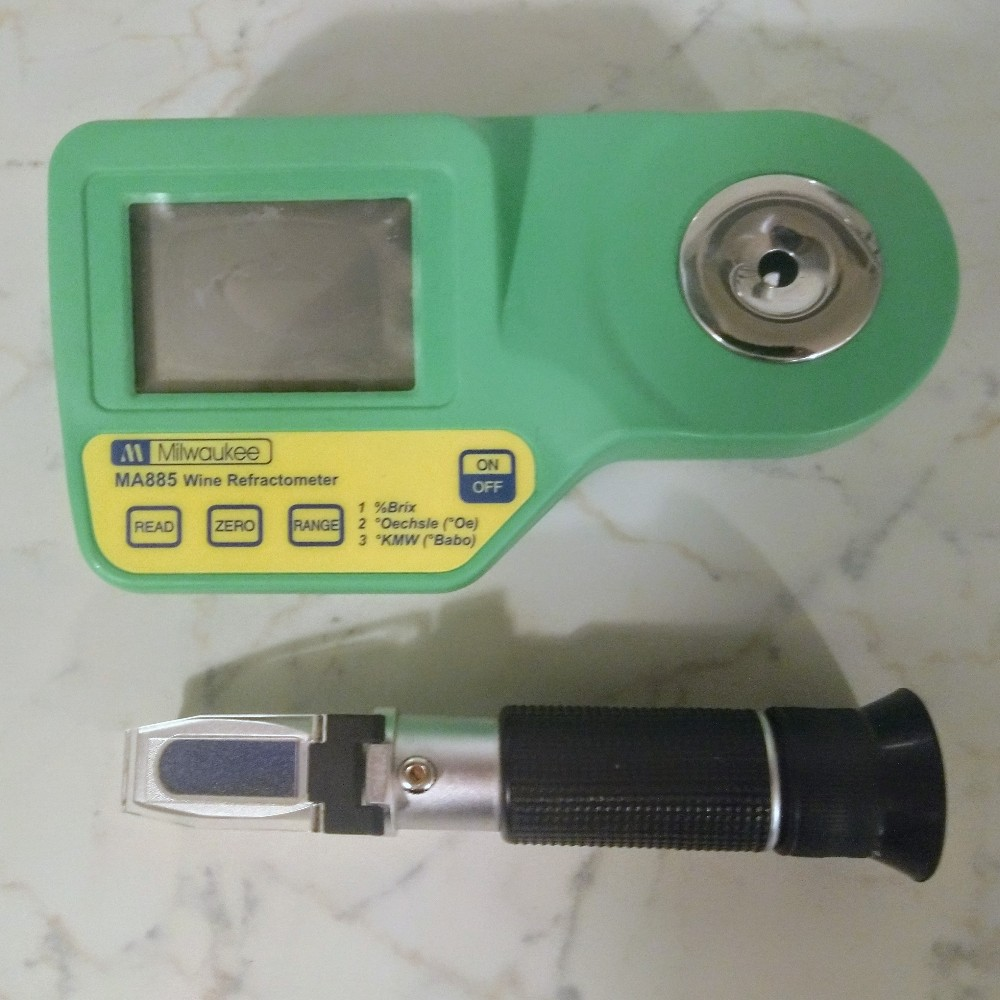
\includegraphics[width=4.8cm]{images/types.jpg}
\caption{Typische Refraktometer im Heimbraubereich (Ascher, 2021)}
\label{fig:refactotype}
\end{figure}

\begin{table}[h]
\centering
\begin{tabular}{lrr}
\toprule
Parameter &  Handrefraktometer &  Milwaukee MA885 \\
\midrule
Preis [€] & 40 & 185 \\
Messbereich [°Bx] & 0--32 & 0--50 \\
Auflösung [°Bx] & 0,2 & 0,1 \\
Genauigkeit [°Bx] & 0,2 & 0,1 \\
ATC [°C] & 10--30 & 10--40 \\
Maßeinheiten & °Bx, SG & °Bx, °Oe, °KWM \\
Kalibrierschein & nein & ja \\
\bottomrule
\end{tabular}
\caption{Spezifikation typischer Refraktometer im Heimbraubereich  (Ascher, 2021)}
\label{table:refactospec}
\end{table}

Tilt Hydrometer
Brewbrain Float
PLAATO Airlock
iSpindel
Grainfather Conical Fermenter Pro
Grainfather Glycol Chiller Adapter
Manuelle Einträge

5 -> 6 phasen
4 profile, neue anlegen

Lower Temperature Alert
Calibration

Firmware Update

\url{https://community.grainfather.com}
Grainfather Community Account

GF Connect App

\section*{Umrüstung}




\section*{Resümee}

Die relevanten Eckpunkte dieses Artikels sind:

\begin{itemize}
\item Refraktometer messen auf Basis der Brechung des Lichts. Im


\end{itemize}


\end{document}